\documentclass{article}

\usepackage{graphicx}
\usepackage{tikz}
\usepackage{tikzsymbols}
\usetikzlibrary{calc,patterns,shapes.geometric}
\pagestyle{empty}
\usepackage[margin=0pt]{geometry}
\geometry{papersize={14in,12in}}

\def\centerarc[#1](#2)(#3:#4:#5){\draw[#1] ($(#2)+({#5*cos(#3)},{#5*sin(#3)})$) arc (#3:#4:#5);}

\begin{document}
	\begin{figure}
		\centering
		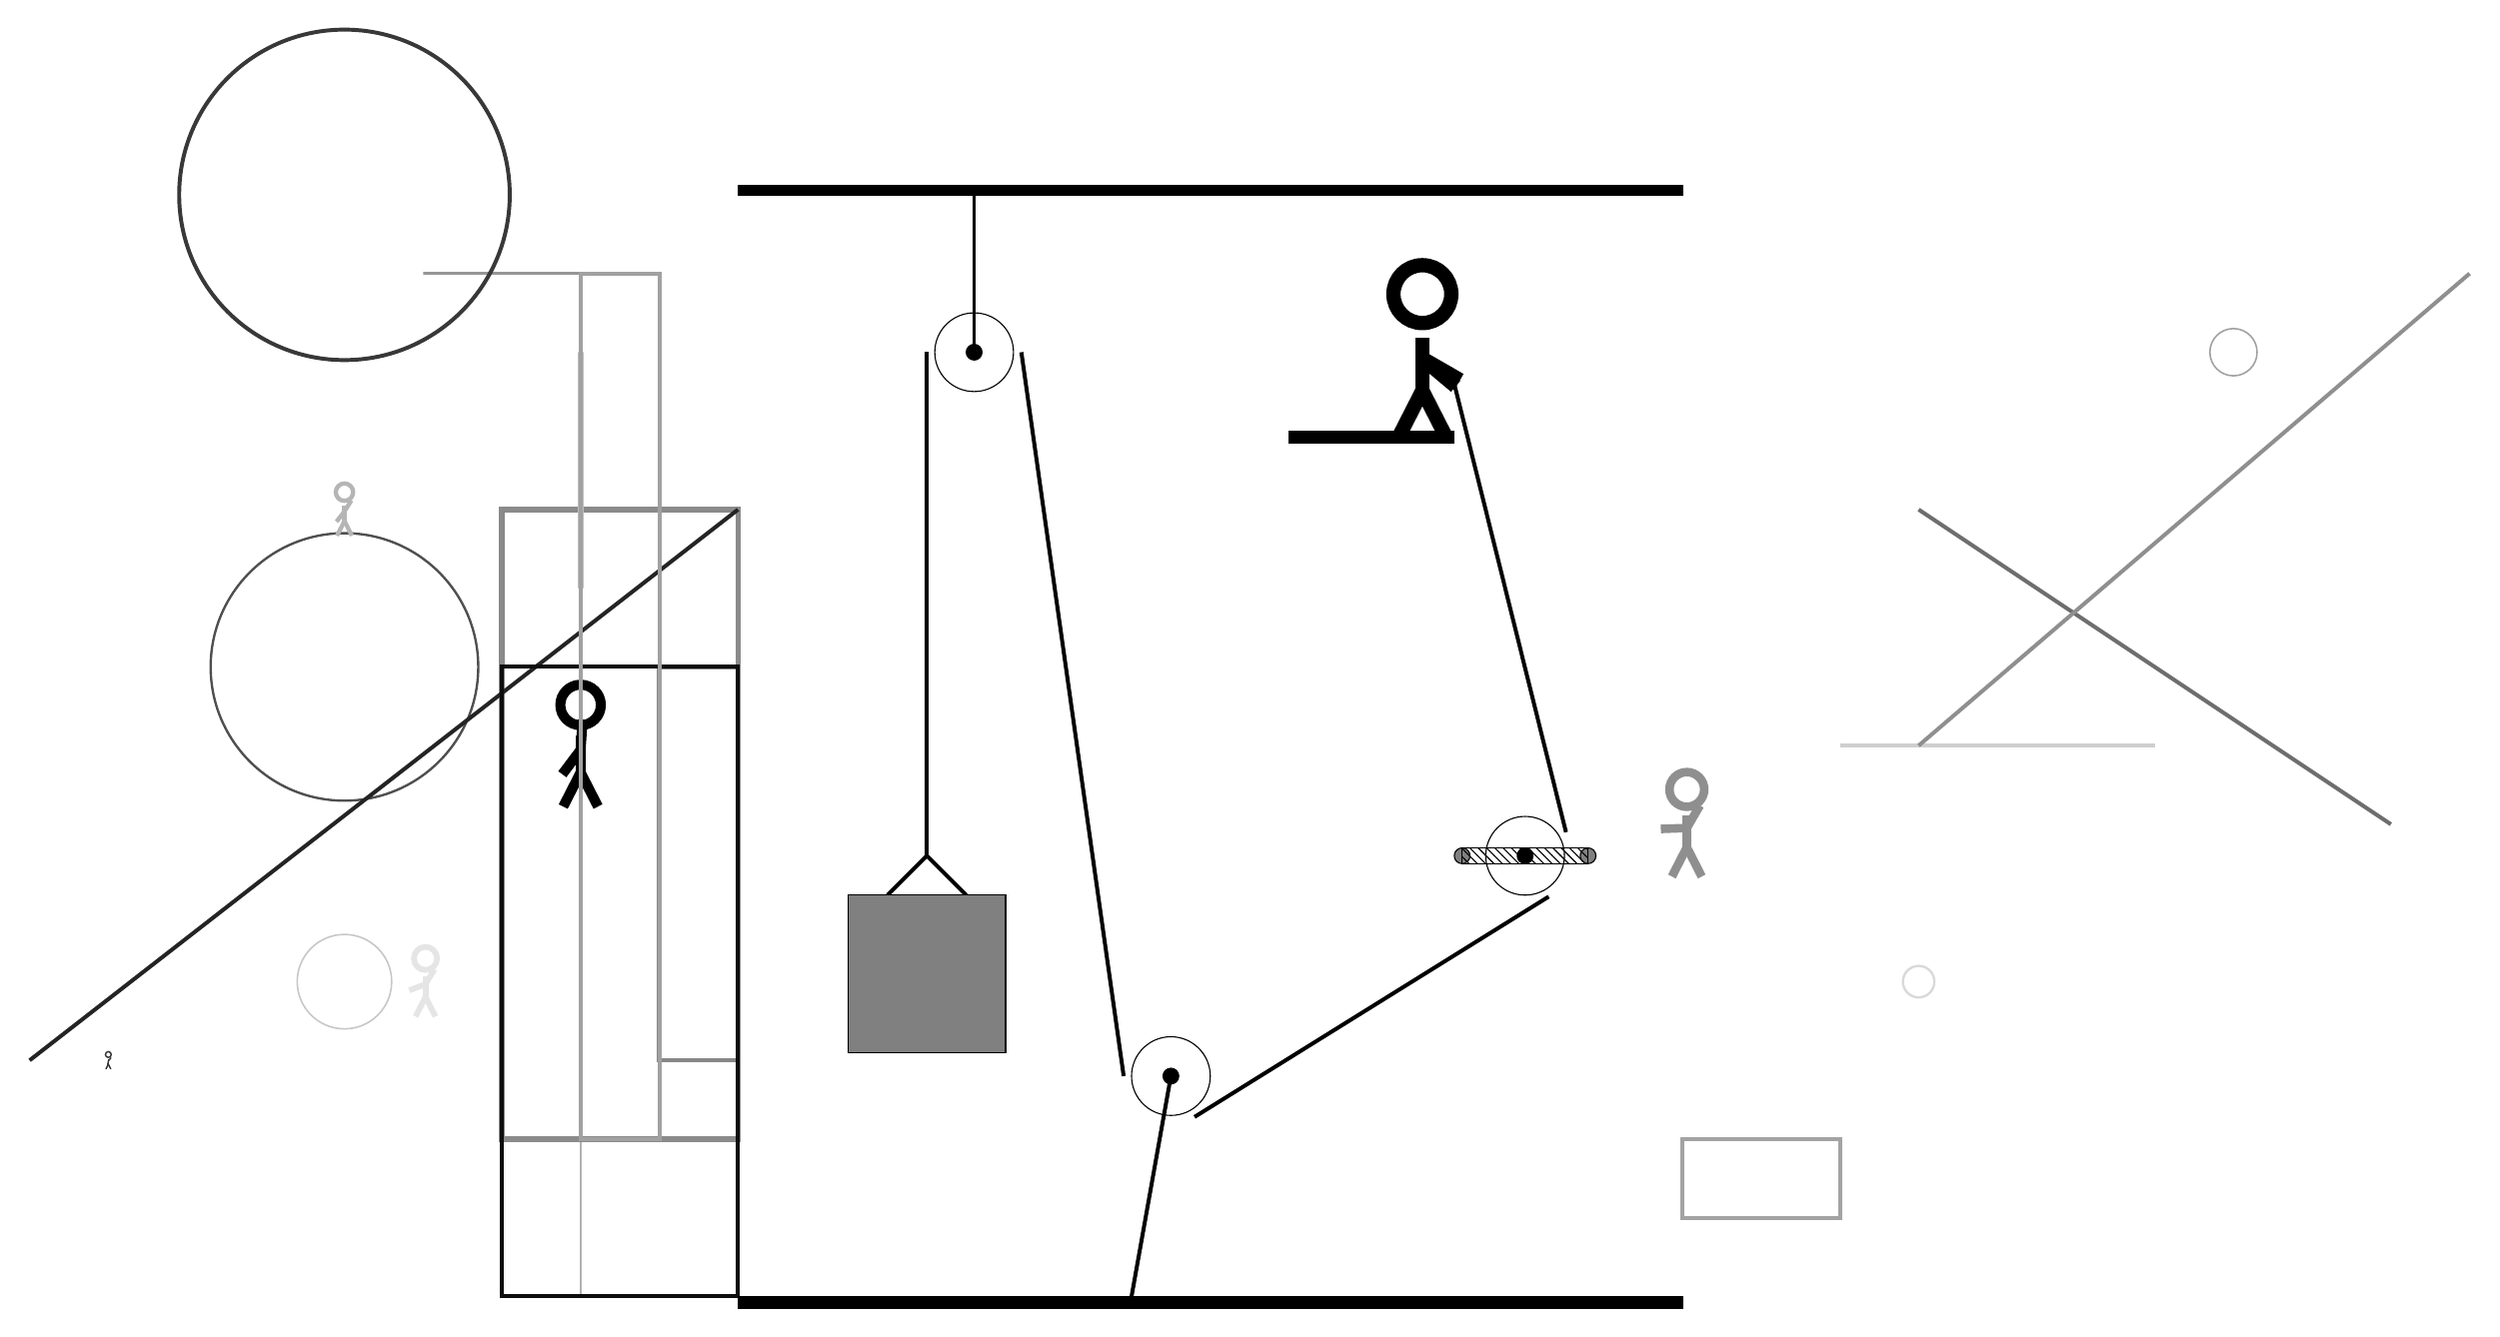
\begin{tikzpicture}
			%%%%% START %%%%%
			
			\draw[fill=black] (-2, 14) rectangle (10, 14.125);
			
			\draw (1, 12) circle (0.5);
			\draw[fill=black] (1, 12) circle (0.1);
			\draw[line width=0.5mm] (1, 14) -- (1, 12);
			
			\draw (3.5, 2.8) circle (0.5);
			\draw[fill=black] (3.5, 2.8) circle (0.1);
			\draw[line width=0.5mm] (3.5, 2.8) -- (3.0, 0);
			
			\draw[line width=0.6mm, color=black!47] (-3, 8) rectangle (-2, 3);
			
			\draw [line width=0.3mm, color=black!15](13, 4) circle (0.2);
			\draw [line width=0.2mm, color=black!37](17, 12) circle (0.3);
			\draw[line width=0.5mm, color=black!19](12, 7) -- (16, 7);
			\draw [line width=0.2mm, color=black!22](-7, 4) circle (0.6);
			\draw[line width=0.3mm, color=black!30] (-4, 10) rectangle (-4, 0);
			
			\draw[line width=0.5mm, color=black!36] (12, 1) rectangle (10, 2);
			\draw [line width=0.3mm, color=black!69](-7, 8) circle (1.7);
			\draw[line width=0.7mm, color=black!46] (-2, 2) rectangle (-5, 10);
			\draw[line width=0.4mm, color=black!41] (-3, 13) rectangle (-6, 13);
			\draw [line width=0.5mm, color=black!78](-7, 14) circle (2.1);
			
			\draw[line width=0.5mm, color=black!86](-2, 10) -- (-11, 3);
			\draw[line width=0.7mm, color=black!26] (-4, 12) rectangle (-4, 9);
			
			\node[line width=0.2mm, color=black!100] at (-4, 7) {\Strichmaxerl[7][53][86]};
			\node[line width=0.5mm, color=black!44] at (10, 6) {\Strichmaxerl[6][2][60]};
			\draw[line width=0.5mm, color=black!95] (-2, 0) rectangle (-5, 8);
			
			\draw[line width=0.5mm, color=black!37] (-4, 2) rectangle (-3, 13);
			\draw [line width=0.7mm, color=black!31](-6, 3) circle (0.0);
			\node[line width=0.5mm, color=black!10] at (-6, 4) {\Strichmaxerl[4][21][59]};
			
			\draw[line width=0.5mm, color=black!57](13, 10) -- (19, 6);
			\node[line width=0.3mm, color=black!29] at (-7, 10) {\Strichmaxerl[3][52][58]};
			
			\draw[line width=0.5mm, color=black!44](13, 7) -- (20, 13);
			\node[line width=0.6mm, color=black!79] at (-10, 3) {\Strichmaxerl[1][81][50]};
			
			\draw[fill=white](8, 5.6) circle (0.5);
			\draw[fill=black] (8, 5.6) circle (0.1);
			\draw[fill=black!50] (8.8, 5.6) circle (0.1);
			\draw[fill=black!50] (7.2, 5.6) circle (0.1);
			\draw[pattern=north west lines, pattern color=black] (7.2, 5.7) rectangle (8.8, 5.5);
			
			\draw[line width=0.5mm](-0.1, 5.1) --  (0.4, 5.6) -- (0.9, 5.1);
			\draw[fill=black!50] (-0.6, 5.1) rectangle (1.4, 3.1);
			
			\draw[line width=0.5mm](0.4, 12) -- (0.4, 5.6);
			\centerarc[line width=0.5mm](1, 12)(180:0:0.6)
			\draw[line width=0.5mm](1.6, 12) -- (2.9, 2.8);
			\centerarc[line width=0.5mm](3.5, 2.8)(180:300:0.6);
			\draw[line width=0.5mm](3.8, 2.2804) -- (8.3, 5.0804);
			\centerarc[line width=0.5mm](8, 5.6)(300:390:0.6);
			\draw[line width=0.5mm](8.5196, 5.9) -- (7.05, 11.8);
			
			\node at (6.75, 12) {\Strichmaxerl[10][-220][-30]};
			\draw[fill=black] (5, 11) rectangle (7.1, 10.85);
			
			\draw[fill=black] (-2, 0) rectangle (10, -0.15);
			
			%%%%% END %%%%%
		\end{tikzpicture}
	\end{figure}	
\end{document}